\chapter{Evaluation and Results}
\section{Dynamic Resource Allocation in a Manycore OS}\label{eval-dynamic}
%	c.	Dynamic System
%		i.	Single Application � right sizing
%			1.	Without phase changes
%			2.	With phase changes
%			3.	Baseline � all allocations
%			4.	Measure Energy
%		ii.	Video, Animation, and Throughput Applications w/o phase changes
%			1.	Show throughput and missed deadlines for all the possible mixes
%			2.	Is it possible to show optimal?
%			3.	What is the baseline?
%		iii.	Video, Animation, and Throughput Applications w/ phase changes
%			1.	Show throughput and missed deadlines for all the possible mixes
%			2.	Basically just to show the system works



\begin{figure*}[!t]
	\begin{center}	
		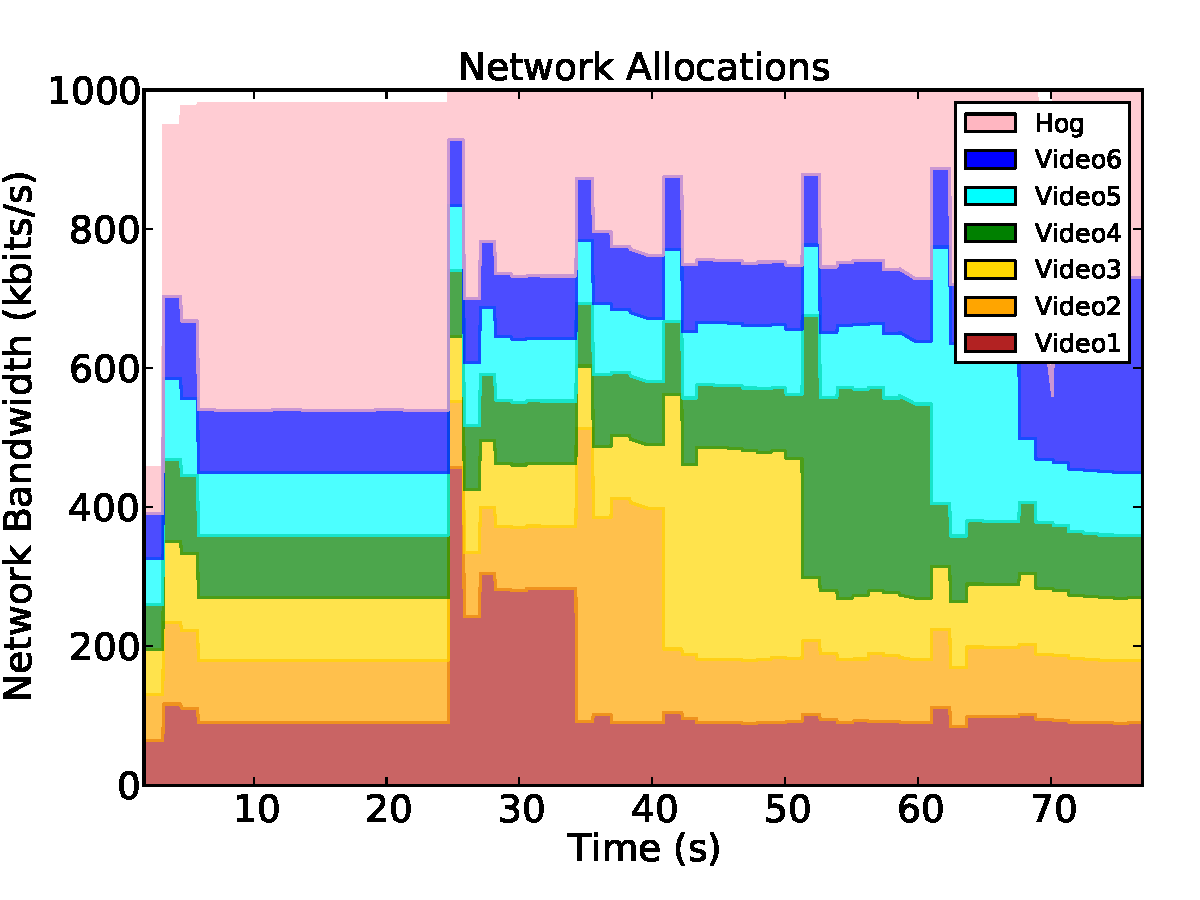
\includegraphics[bb=0 0 576 432,width=.49\textwidth]{Figures/dyn-alloc-wp-ns.pdf}
		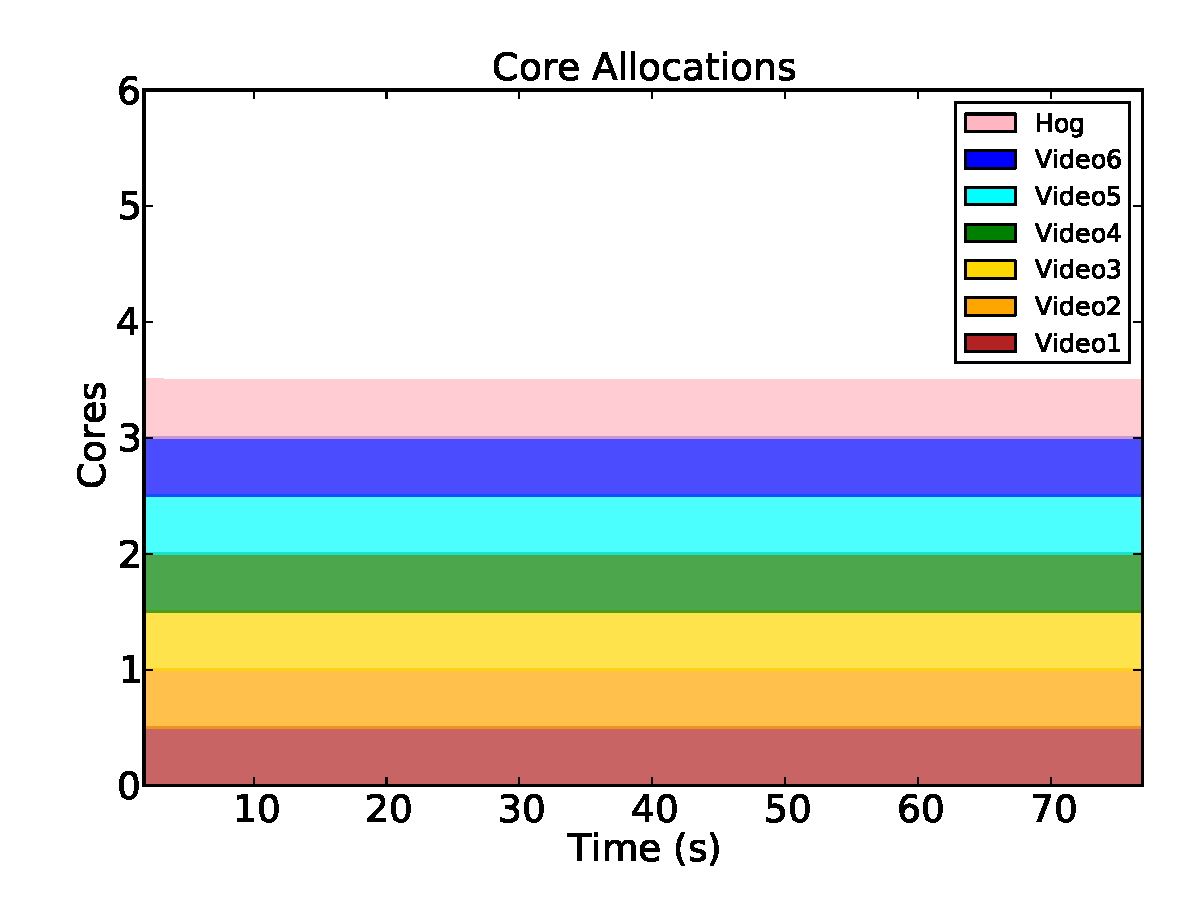
\includegraphics[bb=0 0 576 432,width=.49\textwidth]{Figures/dyn-alloc-wp-core.pdf}
		\caption{Wall Power Mode: Resource Allocations of video conferencing through time as the videos change resolution to adjust for which person is speaking. Hog represents a background task uploading files.}
		\label{video_experiment_wp}
	\end{center}
\end{figure*}

\begin{figure}[!t]
	\begin{center}	
		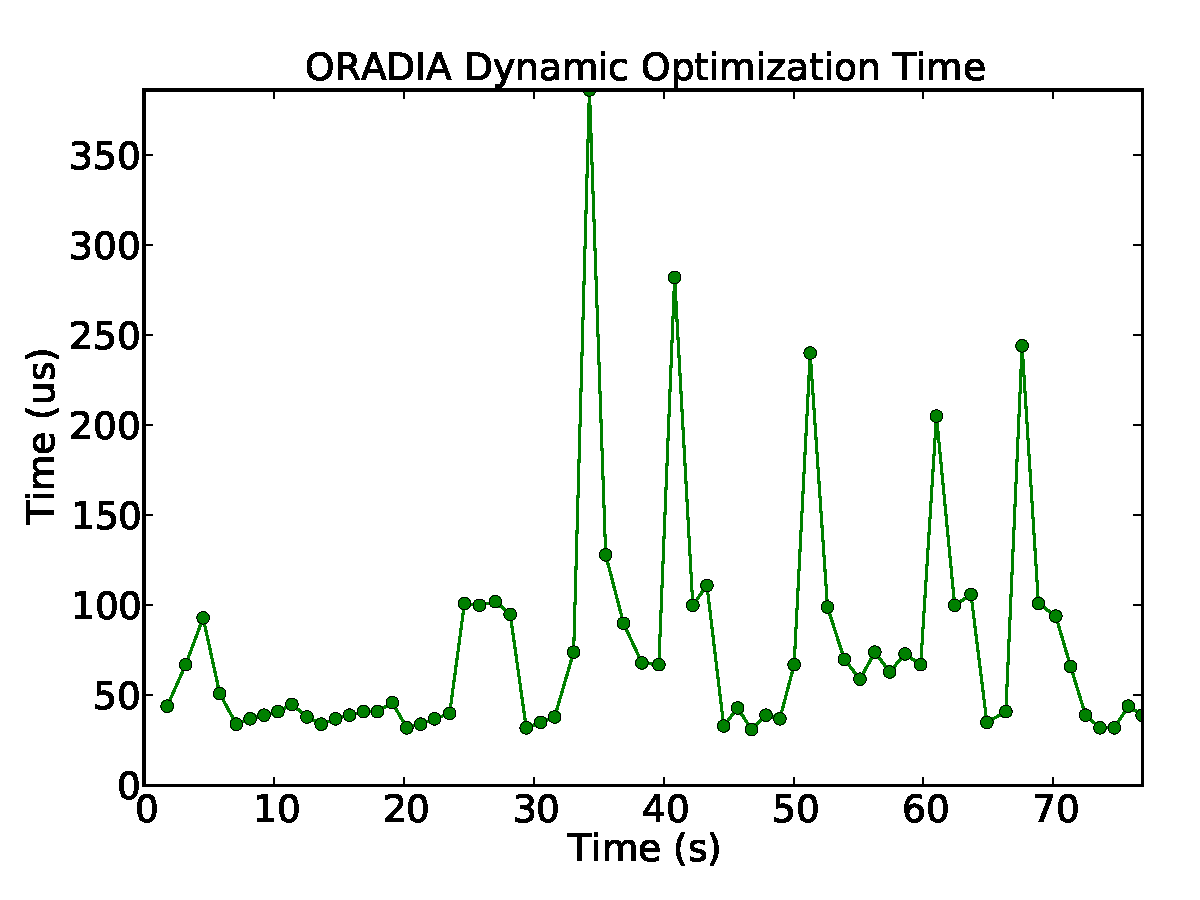
\includegraphics[bb=0 0 576 432,width=\columnwidth]{Figures/opt_time.pdf}
%		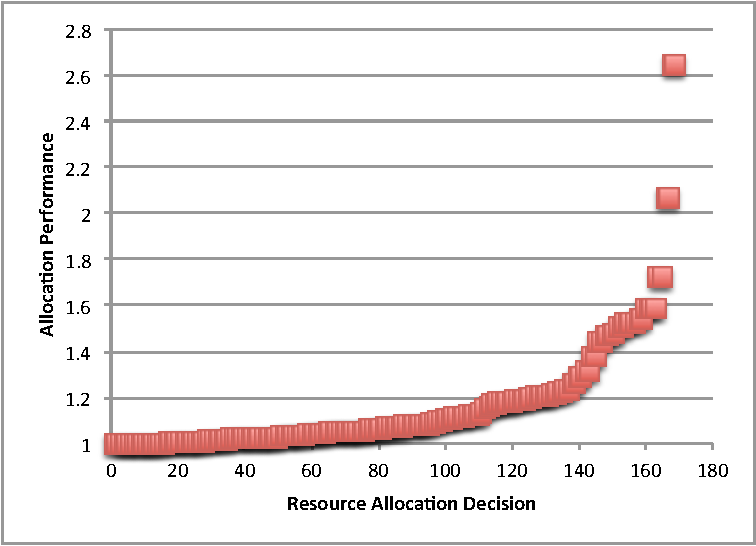
\includegraphics[width=.45\textwidth]{parsec_decision_points.pdf}
		\caption{Performance of our penalty optimization algorithm}
		\label{optimization_perf}
	\end{center}
\end{figure}

\begin{figure}[!t]
	\begin{center}	
		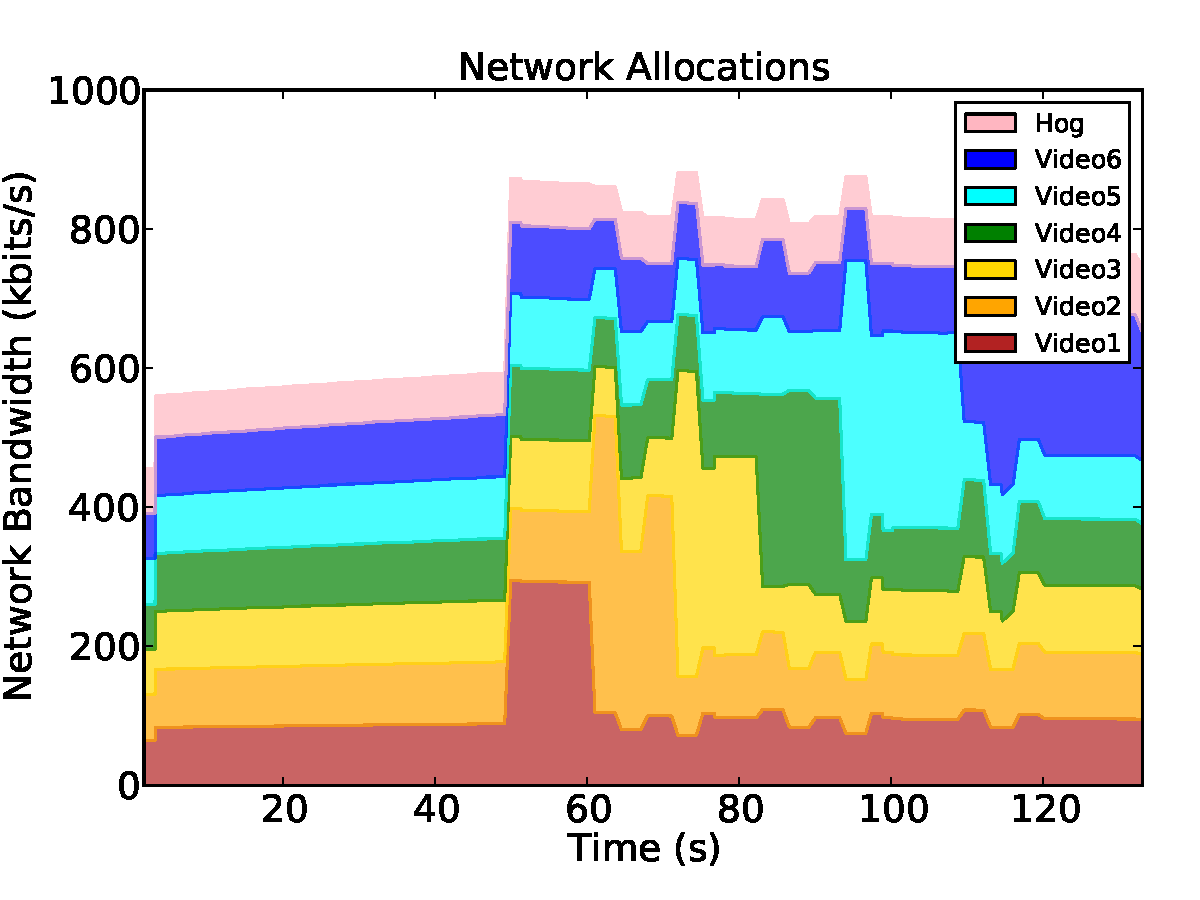
\includegraphics[bb=0 0 576 432,width=\columnwidth]{Figures/dyn-alloc-battery-ns.pdf}
		\caption{Battery Power Mode: Resource Allocations of video conferencing through time as the videos change resolution to adjust for which person is speaking. Hog represents a background task uploading files.}
		\label{video_experiment_battery}
	\end{center}
\end{figure}

%\cite{tess09,tess_dac}

To evaluate \pacora's ability to make real-time decisions in a real operating system, we implemented it in an in-house research operating system, \tess. We chose to implement in \tess rather than Linux for three reasons:
 \begin{enumerate}\itemsep0pt \parskip0pt \parsep5pt
\item \tess separates resource allocation from scheduling, so is
  closer to the OS architecture assumed by \pacora
\item \tess allows resource revocation, enabling \pacora to dynamically reallocate resources
\item \tess implements additional resource partitioning mechanisms,
  letting \pacora manage  more resource types
\end{enumerate}
This dynamic framework is used to test our implementations of the algorithms, measure the overhead and reaction times, and illustrate \pacora's ability to work in a real system.

\subsection{Platform}
Our dynamic experiments are all run on an Intel Nehalem-EP system with two 2.66-GHz Xeon X5550 quad-core processors and hyperthreading enabled with 16 hardware threads. This system also contains a 1-Gbps Intel Pro/1000 Ethernet network adapter.
\tess allocates resources directly to applications, and the applications employ a second-level scheduler to schedule work onto the resources.  
%There are two scheduling frameworks available in \tess: a cooperative framework called Lithe (LIquid THrEads)~\cite{lithe} and a preemptive one called PULSE (Preemptive User-Level SchEduling).  
All of our experiments use a preemptive scheduling framework called PULSE (Preemptive User-Level SchEduling), with two different scheduling strategies: applications with responsiveness requirements use an earliest-deadline-first (EDF) scheduler and throughput-oriented applications use a round-robin (GRR) scheduler.

In addition to allocating cores and cache ways as with our static
framework, \tess can also allocate fractions of network bandwidth.  In
our experiments, we show \pacora allocating cores and network
bandwidth because the experimental platform, which has the advantage
of more cores, does not have cache partitioning.  We have also
successfully experimented with additional resources such as memory pages and CPU
utilization, but the results are not presented here for brevity.

\subsection{Performance and Energy Measurement}

Applications report their own measured response times to \pacora
through a message-passing interface built into \tess, and \pacora uses
this information to build models offline or online.  The online models
are identical to our offline models for the same inputs, so the method
used has no effect on resource allocation decisions.  However, online
models are able to adapt changes in applications.  Modeling is
discussed further in Section~\ref{RTFs}.
%and we also use this information to show if the application is making its deadlines for the experiments.

\tess enables \pacora to directly measure the system energy.  However, energy counters are not available on our Nehalem-EP system and thus we extend the power model from the Sandy Bridge system to function as our application 0 RTF.

\subsection{Description of Workloads}
Our workload is designed to represent a video conference with participants from many remote locations. There is a separate, performance-guaranteed incoming video stream for each participant.
%New participants may join the conference and others may leave, increasing or decreasing the number of streams running at any given time.
The application adjusts video sizes based on which person is
speaking. The speaker's video is larger and has higher resolution than
the other video streams, and as the speaker changes, the requirements
for the video streams change. In the background, network-intensive
tasks such as uploading and downloading files are executed.
%While conferencing, compute-intensive tasks such as virus scans or file indexing could be executed in the background.

Our streaming video application is a multi-threaded, CPU- and
network-intensive workload intended to simulate video chat
applications like Skype and Facetime.  Each video stream is encoded
offline in the H.264 format using libx264, transported across the
network through a TCP connection from a Linux E5-based server, and
decoded and displayed by the \tess client. The client receives,
decodes, and displays each frame using libffmpeg and libx264. Each
video stream has a corresponding EDF-scheduled thread with 33 ms
deadlines using our second-level EDF scheduler.  We also use a network
bandwidth hog application designed to represent an application such as
Google Drive or Dropbox uploading files to the cloud. The hog contends
with the video player for bandwidth by constantly sending UDP messages
to the Linux server.

%We use psearchy~\cite{psearchy}, a parallel text indexer, from MOSBENCH\cite{mosbench} as our file indexing application.



\subsection{Resource Allocation Experiments}

We constrain the available resources in the system for \pacora to 1
Mbit/s network bandwidth and 6 cores to simulate a
resource-constrained system as this is a more challenging resource
allocation problem.

In our experiment the video conference contains 6 incoming video
streams.  At first no one is speaking and thus all the videos are
small.  The person speaking rotates across the incoming videos 1--6,
with the videos resizing around every 10 seconds. We set the deadline
to be 33 ms to represent a frame rate of 30 frames/sec. As this rate,
small videos require 80 to 87 kbits/s depending on the particular
frames. Large videos require 250 to 270 kbits/s.  We assign a moderate
penalty (10.0) for missing the deadline to small videos, and a
significant penalty (50.0) for the large videos.  We assign a small
penalty for the network hog (1.0) with no deadline.

Figure~\ref{video_experiment_wp} shows the resource allocations for our video conference scenario when the computer is using ``wall power''.  We mean wall power to imply that saving power is less critical and thus we assign a low penalty slope to application 0.  \pacora gives 90 kbits/s to small videos, 280 kbit/s to large videos, and the remaining bandwidth is given to the network hog.  Video resizes can be seen as the ``steps'' in the graph: for example, Video1 becomes large at 24 seconds resulting in its allocation increasing from 90 kbits/s to 280 kbits/s.  Video2 becomes large at 33 seconds and Video1 returns to its original size.

Since there is a single set of extreme points in a convex problem
after a sufficient number of iterations, our dynamic algorithm will
produce the same allocations as our static framework. The runtime is
controllable based on the exit conditions of the optimization
algorithm, however earlier exits may result in intermediate
reallocations. We can see intermediate resource allocations (the
``columns'' in the graph) as \pacora transitions for one set of
allocations to another.  If run much longer (50 ms), \pacora can
completely eliminate the intermediate allocations, which may be
appropriate in environments where resource reallocation is expensive
and allocations do not need to be adapted frequently.  It is also
possible to provide guaranteed optimization times of around \SI{20}{
\micro\second}, but at the cost of many more intermediate reallocations.
These results can be found in~\cite{pacora_tr}.We choose this
particular point in the space because we believed it strikes the right
balance between reactivity and reallocation amounts for a client
operating system. Figure~\ref{optimization_perf} shows the runtime of
the optimization algorithm as it makes resource allocation decisions
for the video scenario. The algorithm runs in \SI{50}{\micro\second} on average,
with more significant reallocations taking from 250-\SI{350}{\micro\second}.
Significant changes result in 1-2 intermediate reallocations.  In
\tess, network bandwidth is easily reallocated and thus intermediate
reallocations do not have much overhead.  Core allocations are also
easily adjusted between fractional core amounts.  Careful tuning of
the algorithm parameters could potentially yield additional
performance improvements.

Core allocations are also shown in Figure~\ref{video_experiment_wp}.
Neither application in our scenario can take advantage of additional
compute power thus each optimization results in the same core
allocations for the applications regardless of video size.

Figure~\ref{video_experiment_battery} shows same scenario except the
computer is now using ``battery power'' and thus we have increased the
importance of application 0 (penalty 2.0).  The video applications are
still allocated the necessary amount of resources for each video size.
However, the allocation of the network hog is significantly reduced to
less than 70 kbits/s, and the remaining resources are left idle.



\subsection{Adapting Multiple Resources}
\label{sec:exppacora}

Now we demonstrate how PACORA
can be used to efficiently allocate resources for different parts of the video
conference scenario.
 This Section demonstrates using \pacora as the overall resource
brokerage system, dividing resources between the incoming video streams, a file
indexer, and outgoing network data.

Our test platform is an Intel server containing two 2.66-GHz Xeon X5550
quad-core processors with hyper-threading enabled and a 1-Gbps Intel Pro/1000
Ethernet network adapter. 

\begin{figure*}
\centering
\begin{tabular}{cc}
\subfloat(a)Network allocations for 9 incoming videos{
    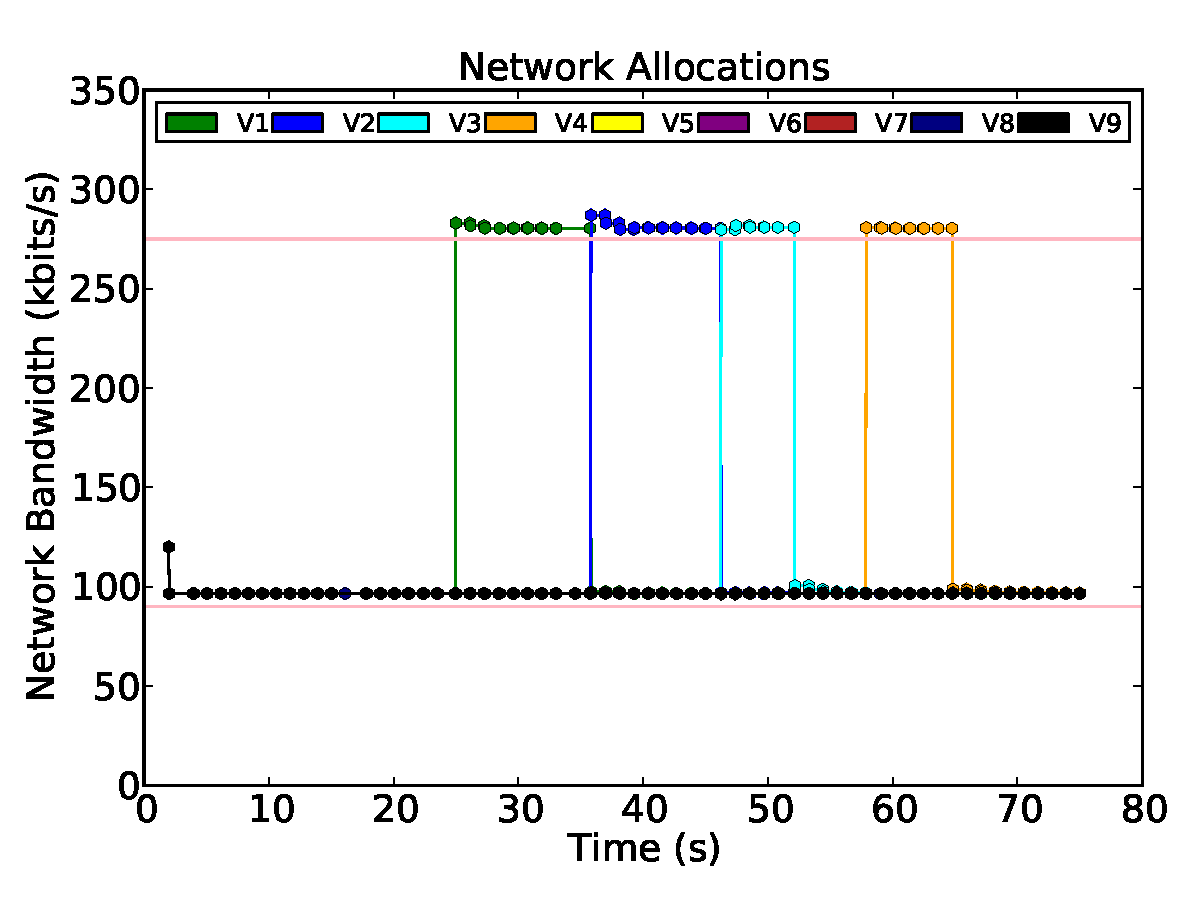
\includegraphics[width=0.45\textwidth]{Figures/NetworkAlloc}
    \label{figures:NetworkAlloc}
   } 
& \subfloat[Network allocations for file indexer and bandwidth hog ]{
    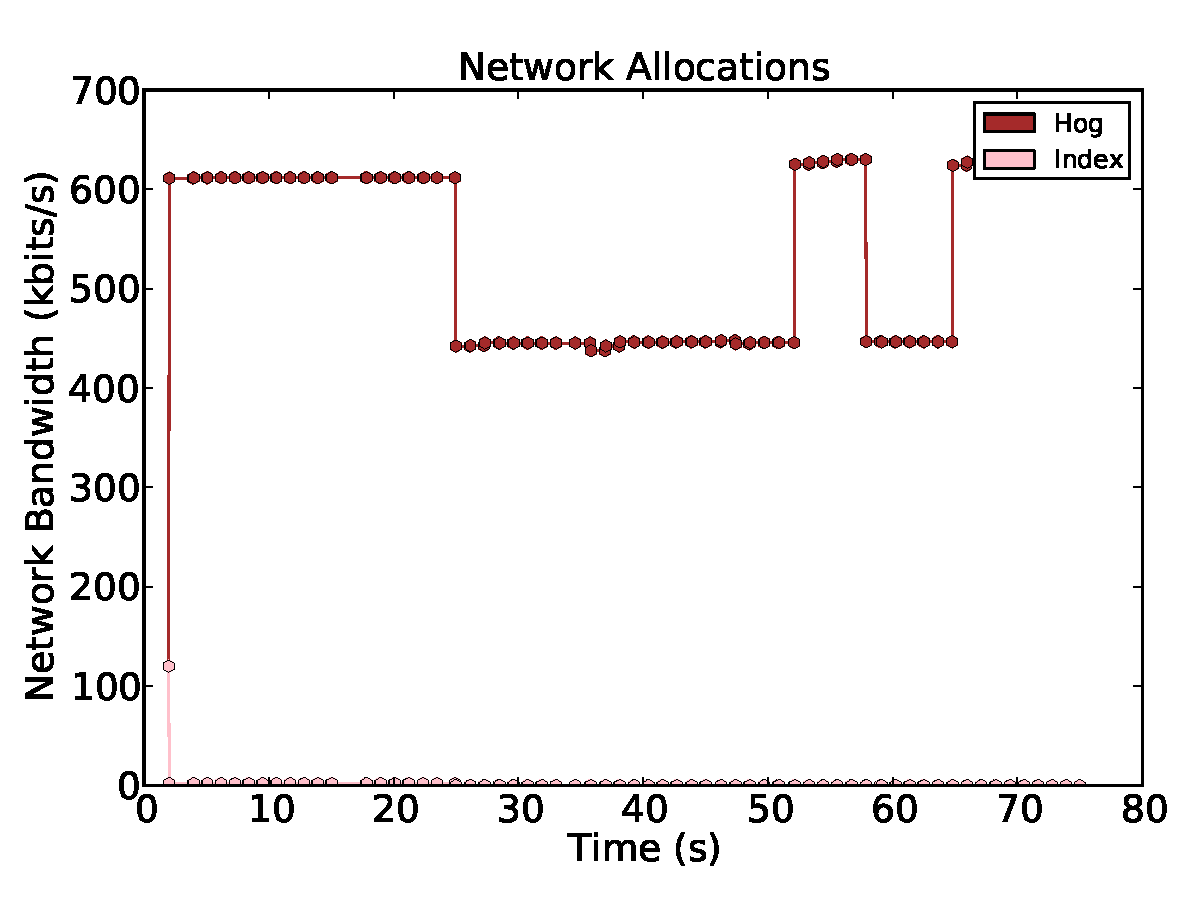
\includegraphics[width=0.45\textwidth]{Figures/HogAlloc}
    \label{figures:HogAlloc}
}\\
\subfloat[Frame rate for 9 incoming videos]{
   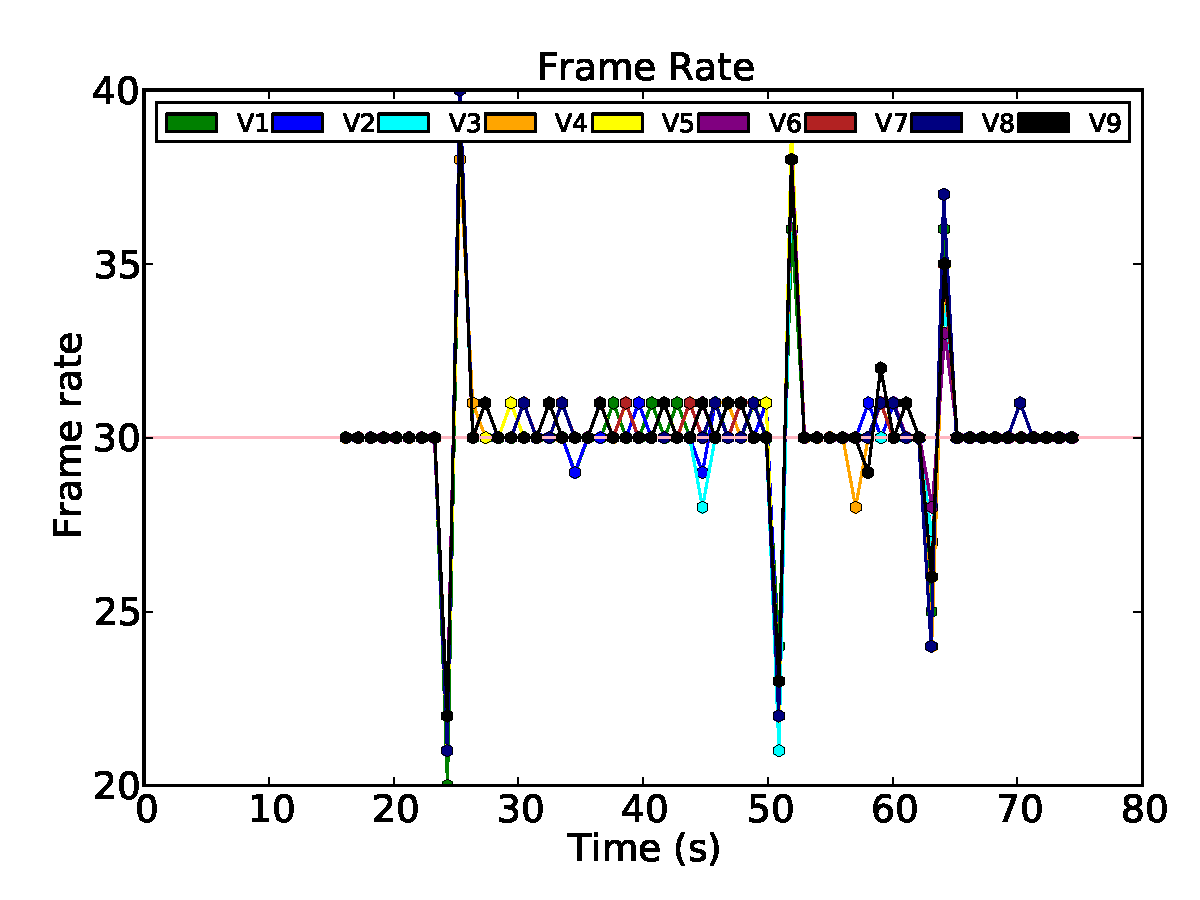
\includegraphics[width=0.45\textwidth]{Figures/Framerate}
    \label{figures:Framerate}
}
& \subfloat[Core allocations for incoming video, file indexer, and bandwidth hog]{
    %\rule{4cm}{3cm}
   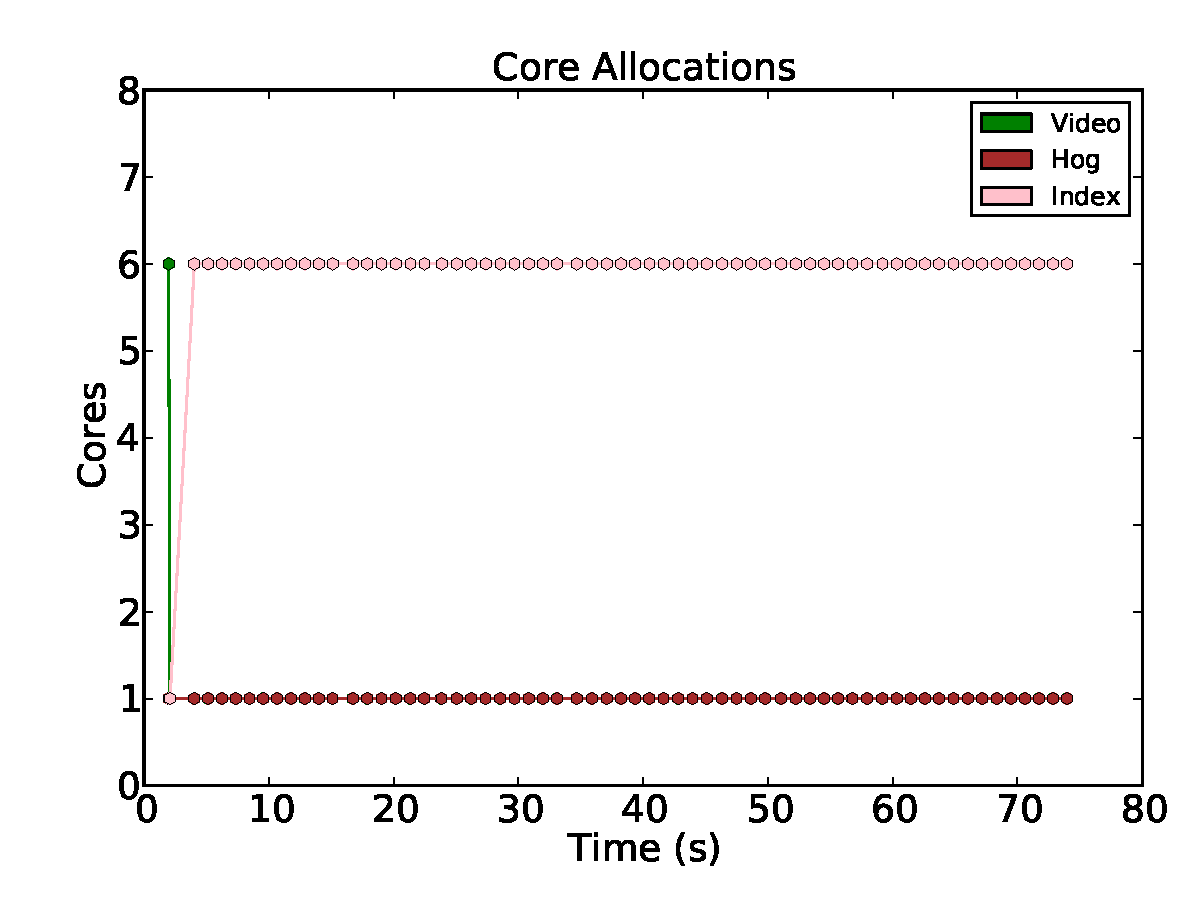
\includegraphics[width=0.45\textwidth]{Figures/CoreAlloc}
    \label{figures:CoreAlloc}
}\\
\end{tabular}
\caption{Allocations and frame rate when running 9 video-player threads, a file
indexer, and a bandwidth hog together.  Periodically, one of the videos becomes large
causing the allocations to change.  The two red lines on
\ref{figures:NetworkAlloc} represent the required network bandwidth for a large
and small video.  The red line on \ref{figures:Framerate} represents the
desired frame rate of 30 fps for the video-player threads.}\label{fig:afexample}
\label{fig:pacora_res}
\end{figure*}

This experiment demonstrates using \pacora to allocate cores and network
bandwidth to 3 applications (video player, file indexer, network hog)
in our video conference scenario and shows our complete adaptive loop in \tess.

Our streaming video application is a multi-threaded, network-intensive workload
intended to simulate video chat applications like Skype and Facetime.
We have 9 incoming video streams each handled by a thread in our video cell,
which uses Pulse EDF scheduler\cite{tess_dac}. 
Each thread receives frames from the network service, decodes them using
libffmpeg, and sends them to the GUI service for display.
Videos are encoded offline in H.264 format using libx264, transported across
the network via a TCP connection from a Linux Xeon E5-based server. 
We use Big Buck Bunny~\cite{bigbuckbunny} for each video. 
Videos can be small or large (although only one may be large at a time)
and are resized by a keyboard command.  
Small videos require roughly 90 kbit/s while large require 275 kbit/s of network
bandwidth.  
\tess provides each video stream a separate network bandwidth allocation, and
the videos share their core allocations using the EDF scheduler.

%% psearchy and the bandwidth hog
Our file indexer application is psearchy, a pthread-based parallel application
from the MOSBENCH benchmark suite~\cite{mosbench}. 
%Psearchy was designed to index and query Web pages, but instead we use the
%Linux 2.4.0 source code.
It runs on top of a pthread-compatible runtime system implemented in Pulse. 
The TCP bandwidth hog is a simple, single-threaded application that transmits
data at the fastest possible rate, similar to Dropbox or an FTP server.



Figure~\ref{fig:pacora_res} shows the allocations of the applications and video
frame rates as \tess runs and adapts to the video resizes.  The first adaptation
event occurs at t= \SI{2}{\second}, when \pacora changes the allocations from their initial
settings to application-specific allocations.  All network allocations were
initially set to 120 kbits/s, and as shown in Figures~\ref{figures:NetworkAlloc}
and \ref{figures:HogAlloc}, \pacora changes all of the video threads to 96
kbits/s, just above the required network bandwidth for small videos.  \pacora removes
all bandwidth from the file indexer since it does not use network bandwidth and
gives the remaining bandwidth in the system to the network hog\footnote{We have
artificially limited the available cores to 8 and the available network
bandwidth to 1500 kbits/s to make the resources more constrained.}.  We also see
in Figure~\ref{figures:CoreAlloc} that \tess removes cores from the video cell
and gives them to the file indexer, utilizing the mechanisms described in \cite{tess_dac} to do so. 


Additional resizing events occur at 25, 35, 52, 58 and 65 seconds, when videos
1, 2, 3, and 4 change size.  As shown in Figures~\ref{figures:NetworkAlloc} and
\ref{figures:HogAlloc}, \pacora reduces the network hog's allocation in order to
give sufficient bandwidth to the large video.  However, when all the videos are
small the bandwidth is returned to the network hog.  
Figure~\ref{figures:CoreAlloc} shows that larger videos do not need enough additional
processing power to require an increase in cores, so the core allocations do not
change after the initial adaptation. Figure~\ref{figures:Framerate} shows that
the videos do not drop below the required frame rate except when
resizing\footnote{Glitches while resizing are an artifact of the application
implementation.}. 

All of the runtime functions used in this experiment were built automatically
from measured values using The Resource Broker's heartbeat interface. These results
demonstrate that using \tess's kernel, Pulse, and the Resource Broker, we are able
to implement a resource-allocation approach that can efficiently assign
resources to applications and adapt the resource allocations as the system
changes state.  As a result using an ARCC style system, we do not need to
sacrifice utilization in order to provide performance guarantees. 




